\begin{abstract}
En este proyecto se implementa un sistema que controle el estado de un conjunto de bombillos a través de gestos.  La primera funcionalidad consiste en que el sistema permitirte elevar y disminuir la intensidad de la luminaria desde completamente apagado, hasta la intensidad máxima. Por otra parte, se implementa un algoritmo que operará por defecto, encendiendo y cambiando la intensidad de las luces en función de la hora del día. El flujo bajo el cual se modela dicho sistema se muestra en la figura \ref{diagrama}. El primer elemento que se puede observar de izquierda a derecha es una cámara, la cual enviará su transmisión al segundo componente: una computadora. La PC ejecutará un programa de reconocimiento de imágenes, el cual procesará la transmisión de la cámara. Si el programa detecta alguno de los gestos definidos, se enviará una respuesta al tercer componente: un Arduino UNO. Con base en el estímulo recibido, este microcontrolador generará la combinación de salidas correspondiente para producir el resultado deseado, ya sea encender, apagar, atenuar o aumentar el brillo del bombillo. Finalmente, el cambio en las salidas se propagará por un circuito de control que manipula la tensión suministrada al bombillo, y consecuentemente variará su intensidad luminosa. El proyecto entrega resultados satisfactorios en todo los puntos deseados.


\end{abstract}

Repositorio en GitHub: \faGithub   \hspace{0.5mm}\url{https://github.com/Jams1001/IE0624/tree/main/Poyecto} 

\texttt{ID del último commit de interés:\href{https://github.com/Jams1001/IE0624/commit/e96a6fcf3fcca333e339f4346ee823d04a5a9c9e}{xd
}}\\

%\keywords{FEM}
\begin{figure}[H]
\centering
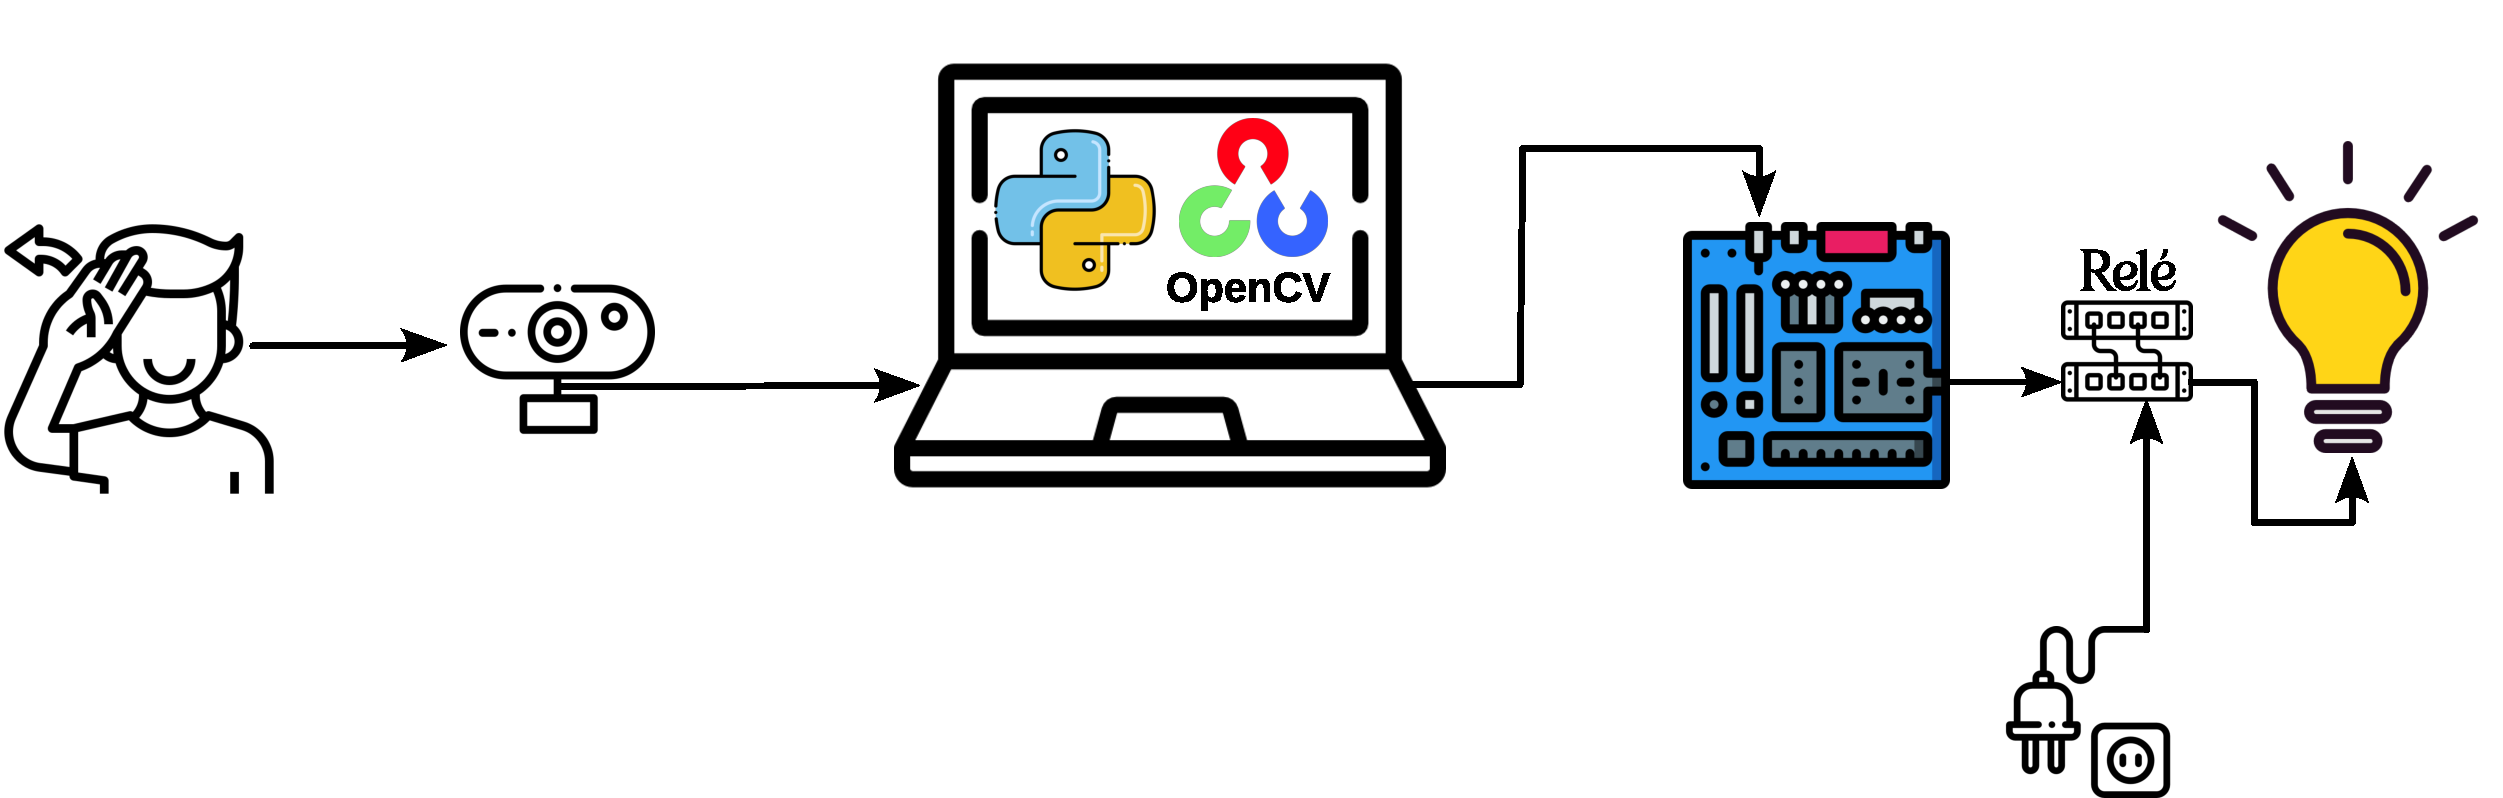
\includegraphics[scale=0.4]{./images/diagrama.pdf} 
\caption{Diagrama ilustrativo (Autoría Propia).}
\label{diagrama}
\end{figure}
